
\documentclass[11pt]{article}
\usepackage[margin=0.78in]{geometry}
\usepackage{booktabs}
\usepackage{array}
\usepackage{graphicx}
\usepackage{float}
\usepackage{hyperref}
\hypersetup{colorlinks=true, linkcolor=blue, urlcolor=blue}
\setlength{\parskip}{0.45em}
\setlength{\parindent}{0pt}
\renewcommand{\arraystretch}{1.12}

\title{Profitability Stress Tests\\\large Rolling ML TP2 Strategy Selection}
\author{ML-Based Trading of TP2-Inspired Violations in SPY American Call Options}
\date{June 22, 2026}

\begin{document}
\maketitle

\section{Purpose}

This report stress-tests the rolling LightGBM selected trades. It does not
retrain the models. Instead, it takes the selected test trades and checks
commission sensitivity, tail dependence, concentration, and drawdown.

\section{Aggregate Selected-Trade Diagnostics}
\begin{tabular}{lrrrrrrrrr}
\toprule
Gate & Selected & Executed & Invalid & Hit rate & Net P\&L & Median executed P\&L & Max drawdown & Top 1\% share & Top 5\% share \\
\midrule
Base & 14,874 & 8,672 & 6,202 & 50.3\% & \$1.99M & \$0 & -\$1.23M & 90.6\% & 221.1\% \\
Volume + Delta & 1,865 & 1,720 & 145 & 55.2\% & \$5.7K & \$9 & -\$156.4K & 2401.3\% & 5071.4\% \\
Strict Quality & 1,650 & 1,489 & 161 & 61.3\% & \$195.0K & \$25 & -\$77.7K & 53.8\% & 125.3\% \\
\bottomrule
\end{tabular}

\section{Commission Stress}
\begin{tabular}{lrrrr}
\toprule
Gate & Commission & Executed & Hit rate & Net P\&L \\
\midrule
Base & \$0.65 & 8,672 & 50.3\% & \$1.99M \\
Base & \$1.00 & 8,672 & 48.4\% & \$1.87M \\
Base & \$1.50 & 8,672 & 46.5\% & \$1.69M \\
Base & \$2.00 & 8,672 & 44.9\% & \$1.51M \\
Volume + Delta & \$0.65 & 1,720 & 55.2\% & \$5.7K \\
Volume + Delta & \$1.00 & 1,720 & 52.4\% & -\$14.6K \\
Volume + Delta & \$1.50 & 1,720 & 49.9\% & -\$43.5K \\
Volume + Delta & \$2.00 & 1,720 & 46.7\% & -\$72.4K \\
Strict Quality & \$0.65 & 1,489 & 61.3\% & \$195.0K \\
Strict Quality & \$1.00 & 1,489 & 58.0\% & \$177.4K \\
Strict Quality & \$1.50 & 1,489 & 54.6\% & \$152.2K \\
Strict Quality & \$2.00 & 1,489 & 51.3\% & \$127.0K \\
\bottomrule
\end{tabular}
\begin{figure}[H]
  \centering
  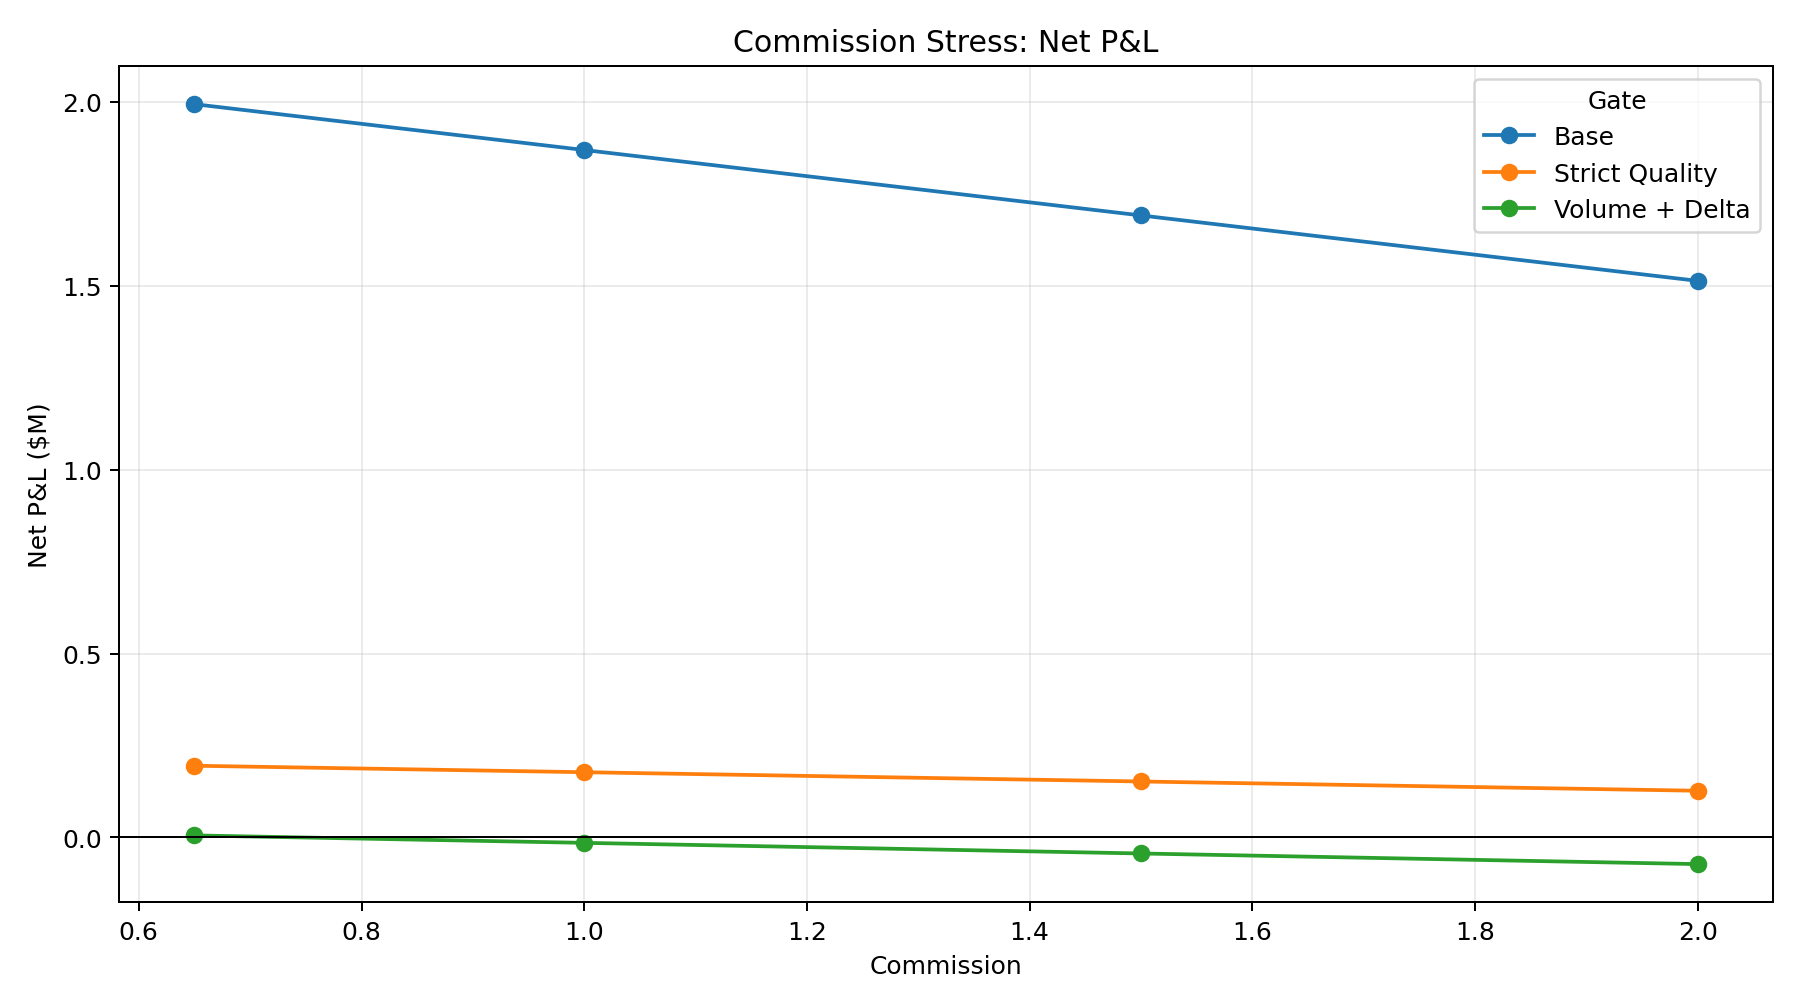
\includegraphics[width=0.92\linewidth]{figures/profitability_stress_commission.png}
  \caption{Net P\&L under higher per-contract per-side commission assumptions.}
\end{figure}


\section{Tail Stress}
\begin{tabular}{llr}
\toprule
Gate & Stress & Net P\&L \\
\midrule
Base & Original & \$1.99M \\
Base & Remove top 1\% executed trades & \$186.6K \\
Base & Remove top 5\% executed trades & -\$2.41M \\
Base & Winsorize 1/99\% & \$2.17M \\
Base & Winsorize 5/95\% & \$1.78M \\
Volume + Delta & Original & \$5.7K \\
Volume + Delta & Remove top 1\% executed trades & -\$130.1K \\
Volume + Delta & Remove top 5\% executed trades & -\$281.1K \\
Volume + Delta & Winsorize 1/99\% & -\$6.0K \\
Volume + Delta & Winsorize 5/95\% & \$13.4K \\
Strict Quality & Original & \$195.0K \\
Strict Quality & Remove top 1\% executed trades & \$90.0K \\
Strict Quality & Remove top 5\% executed trades & -\$49.4K \\
Strict Quality & Winsorize 1/99\% & \$197.6K \\
Strict Quality & Winsorize 5/95\% & \$227.8K \\
\bottomrule
\end{tabular}
\begin{figure}[H]
  \centering
  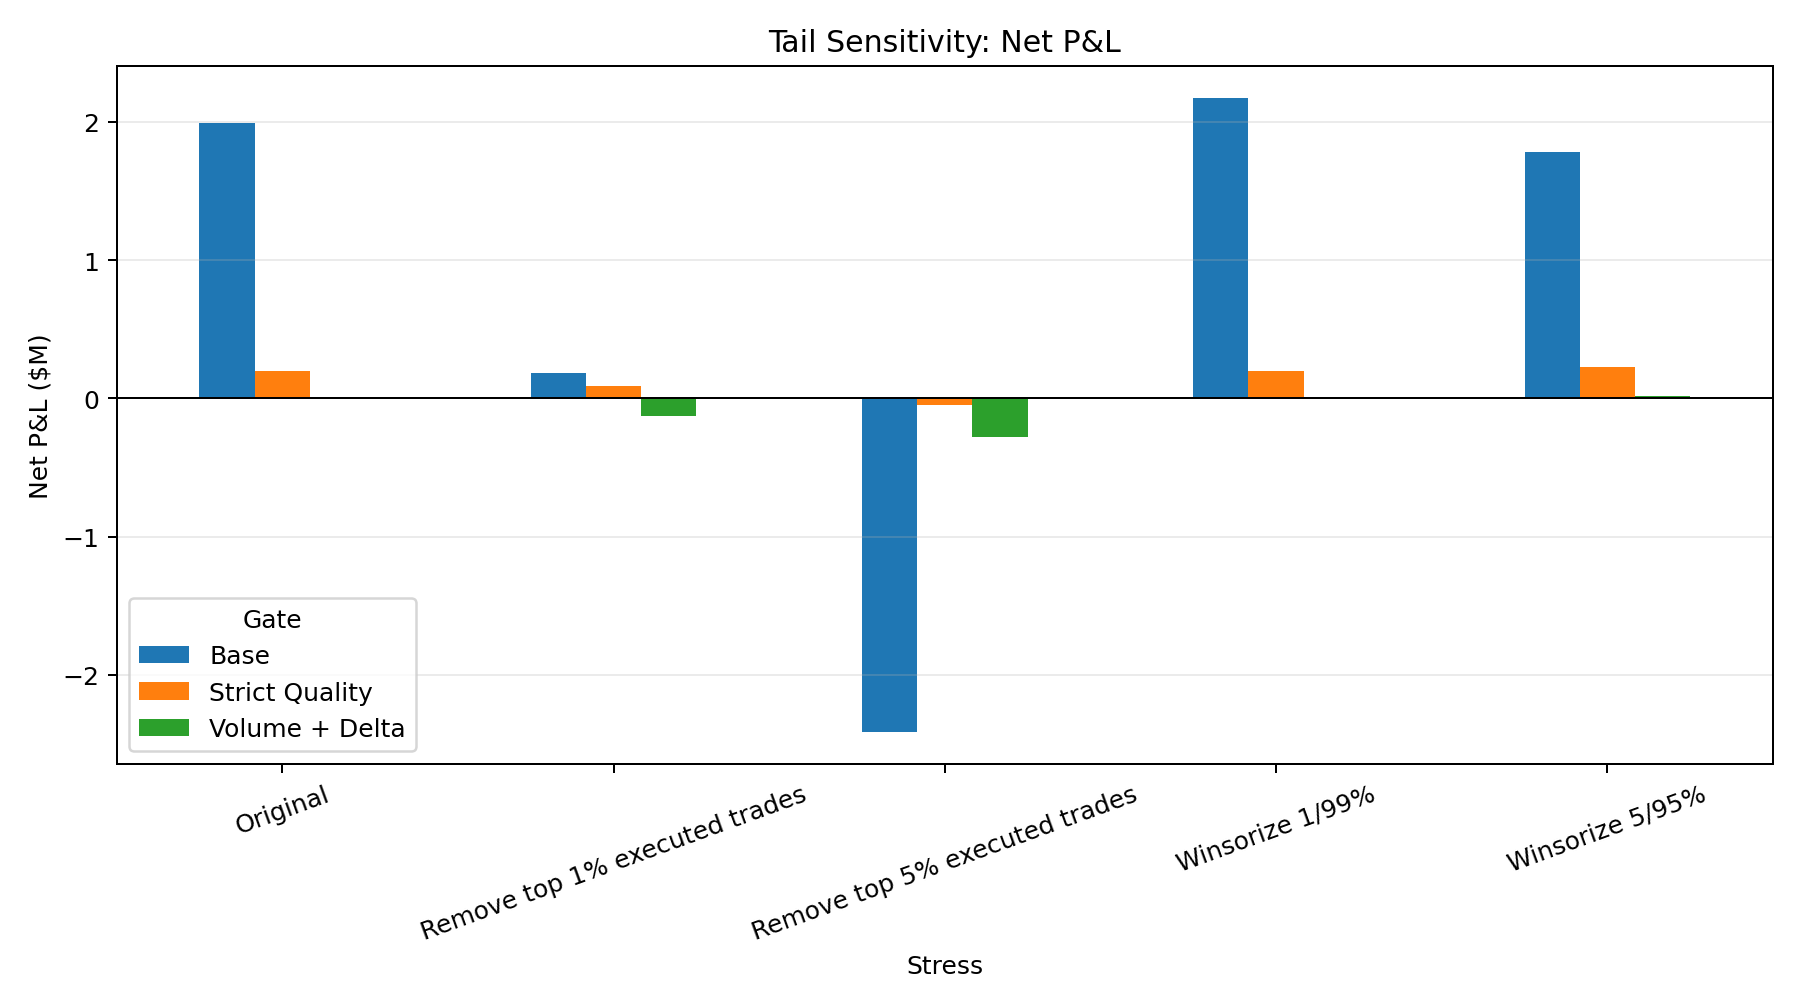
\includegraphics[width=0.92\linewidth]{figures/profitability_stress_tail.png}
  \caption{Net P\&L after removing or winsorizing top executed-trade tails.}
\end{figure}


\section{Interpretation}

The main paper result should not rely only on aggregate P\&L. Concentration,
drawdown, and tail sensitivity must be reported next to the rolling ML results.
If top-tail removal destroys the base result, the paper should frame the model
as identifying rare high-convexity TP2 episodes rather than producing a smooth
market-neutral edge. Filtered universes improve hit rate and execution quality,
but their smaller opportunity set naturally reduces total P\&L.

\end{document}
